\documentclass[a4paper, oneside]{discothesis}

% use utf8 instead of latin1 when using LaTeX in windows
\usepackage[latin1]{inputenc}
\usepackage{mathtools}
\usepackage{comment}
\usepackage{makecell}
\DeclareMathOperator*{\argmax}{\operatorname{argmax}}

%%%%%%%%%%%%%%%%%%%%%%%%%%%%%%%%%%%%%%%%%%%%%%%%%%%%%%%%%%%%%%%%%%%%%%%%%%%%%%%%%%%%%%%%%%%%%%%%%
% DOCUMENT METADATA

\thesistype{Master Thesis}
\title{Adaptive Hierarchical Deep Reinforcement Learning}

\author{Florian Frei}
\email{flofrei@student.ethz.ch}
\institute{Distributed Computing Group \\[2pt]
Computer Engineering and Networks Laboratory \\[2pt]
ETH Z�rich}

% You can put in your own logo here "\includegraphics{...}" or just comment the command
\logo{}

\supervisors{Gino Brunner, Oliver Richter\\[2pt] Prof.\ Dr.\ Roger Wattenhofer}

% You can comment the following two commands if you don't need them
% \keywords{Keywords go here.}
% \categories{ACM categories go here.}

\date{\today}

%%%%%%%%%%%%%%%%%%%%%%%%%%%%%%%%%%%%%%%%%%%%%%%%%%%%%%%%%%%%%%%%%%%%%%%%%%%%%%%%%%%%%%%%%%%%%%%%%

\begin{document}

\frontmatter % do not remove this line
\maketitle

\cleardoublepage

\begin{acknowledgements}
I would first like to thank my thesis advisors Oliver Richter and Gino Brunner of the Distributed Computing Group at Swiss Federal Institute of Technology Zurich.  

The door to Prof. [Last name] office was always open whenever I ran into a trouble spot or had a question about my research or writing. He/She consistently allowed this paper to be my own work, but steered me in the right the direction whenever he thought I needed it.

I would also like to acknowledge David Haldimann a student colleague of mine at Swiss Federal Institute of Technology Zurich as the second reader of this thesis, and I am gratefully indebted for his very valuable comments on this thesis.

Finally, I must express my very profound gratitude to my parents for providing me with unfailing support and continuous encouragement throughout my years of study and through the process of researching and writing this thesis. This accomplishment would not have been possible without them. Thank you.

Florian Frei
\end{acknowledgements}


\begin{abstract}
	smart short recapitulation of stuff done
	main work experiments with temporal abstraction and their adaptability 
\end{abstract}

\tableofcontents

\mainmatter % do not remove this line

%Main reference deep learning \cite{goodfellow2016deep}
%Proximal Policy Approximation for OpenAI five \cite{schulman2017proximal}

\chapter{Introduction}
In 2017 an artificial intelligence named Alpha Go \cite{silver2017mastering} beat the worlds known strongest player in a well-known Japanese board game named Go. This was achieved without using human knowledge but rather the algorithm learned by playing against itself. This type of learning by playing against itself, or in an environment, in machine learning is called reinforcement learning(RL). Another well-known success is from 2015 where the deep Q-network(DQN) algorithm from Mnih et al. (2015) \cite{mnih2015human} learned to play the Atari games from Nintendo only by using pixel input. Both algorithms used the well-known neural networks described in deep learning and combined it with reinforcement learning. This approach is known as deep reinforcement learning(DRL). Because of these successes there is potential in using DRL for learning something more complex such as driving a car. During driving actions such as changing of gear is often repeated in time. Hence it makes sense to introduce a hierarchy for these temporal reoccurring actions to increase learn efficiency. This is studied in the field of hierarchical reinforcement learning(HRL). An algorithm which combines hierarchies with deep reinforcement learning is the option-critic architecture from Bacon et al. (2017) \cite{bacon2017option}. In this work we want to test the \emph{adaptability} and \emph{limitations} of this option-critic architecture and the effectiveness of deliberation cost from Harb et al. (2017) \cite{harb2017waiting}. The option-critic architecture is based on the well-known Asynchronous Advantage Actor-Critic(A3C) algorithm in DRL from Mnih et al. (2016) \cite{mnih2016asynchronous} which is capable of learning navigation in a 3-dimensional random maze from visual input.

\section*{Background}
For the basic knowledge in deep learning such as neural networks we refer to the book from Goodfellow et al. (2016) \cite{goodfellow2016deep} as an introduction and we will assume the reader has a basic understanding of its content. As an introduction into deep reinforcement learning, as already mentioned, we recommend reading about the algorithms such as DQN \cite{mnih2015human} and A3C \cite{mnih2016asynchronous}. To learn more about recent advances in hierarchical reinforcement learning we refer to Bartos et al. (2003) \cite{barto2003recent}.

\section*{Related Work}
The idea of using a hierarchy in reinforcement learning to increase efficiency is well established. The first approach was to define macro actions or operators which can be invoked instead of just basic actions. The first three real frameworks which are still used today were proposed in the nineties. These three major frameworks were the options framework of Sutton et al. (1999) \cite{sutton1999between}, the HAM(hierarchical abstract machines) framework of Parr et al. (1998) \cite{parr1998reinforcement}, and the MaxQ framework of Dietterich (2000) \cite{dietterich2000hierarchical}.

\chapter{Preliminaries}
A finite discounted Markov Decision Process(MDP) $\mathcal{M}$ is a tuple $\mathcal{M} \doteq \\ (\mathcal{S},\mathcal{A},\gamma,r,P)$ encapsulating a state space $\mathcal{S}$, an action space $\mathcal{A}$, a discount factor $\gamma$ where $\gamma \in [0,1)$, a reward function $r(s,a): \mathcal{S} \times \mathcal{A} \to \mathbb{R}$ which maps a state-action pair to a real number and a state transition probability function $P(s,a):\mathcal{S} \times \mathcal{A} \to \mathcal{S} $ which maps states and actions to new states.\\
The behavior is commonly captured by a policy $\pi(s) : \mathcal{S} \to \mathcal{A} $. In a deterministic setting the action taken is always the same given the same state. In a stochastic setting the policy $\pi(a | s) : \mathcal{S} \times \mathcal{A} \to [0,1]$ is a probability distribution over actions given a state.\\
For each action in a given state $s$ the environment returns a reward $r(s,a)$. Based on a policy $\pi$ and reward $r$, a value function can be defined as follows given start state $s$:
\begin{equation*}
V^{\pi}(s) = \mathbb{E} \left[ \sum_{t=0}^{\infty} \gamma^{t} R_t(s_t,a=\pi(s_t)) \right]
\end{equation*}
This value can be used to compare different policies given start state $s$. With the same concept in mind a value can be calculated when the first action is additionally separated from the rest of the policy. This yields a state-action value function $Q_{\pi}(s,a):\mathcal{S}\times\mathcal{A} \to \mathbb{R}$ which can be used to compare different initial actions $a$ from a given start state $s$. If we can calculate values for given states or state-action pairs we also can define a policy based on these values. A well-known policy based on the state-action value function $Q$ is the $\varepsilon$-greedy policy. This policy takes with $\varepsilon$ probability a random action otherwise the action with the maximum $Q$-value is chosen. This is described mathematically as follows:
\begin{equation*}
\pi_{\varepsilon} = \begin{cases}
				  a \sim U_{\mathcal{A}} & \text{if} \; 0<p<\varepsilon<1 \\
				  \displaystyle \max_{a \in \mathcal{A}}{Q(s,a)} &\text{if} \;  0<\varepsilon<p<1 	
			     \end{cases} \qquad p \sim U_{(0,1)}
\end{equation*} where $U_{\mathcal{A}}$ is the uniform distribution over actions and $p$ is a number sampled from an uniform distribution over $(0,1)$.\\
In general, a policy $\pi$ is dependent on parameters $\theta$ which for example describe the distribution. Hence the goal in reinforcement learning is to optimize the policy parameters $\theta$ so that the expected discounted return
\begin{equation*}
 J (\theta) = V^{\pi_{\theta} }(s) =  \mathbb{E} \left[ \sum_{t=0}^{\infty} \gamma^{t} R_t(s_t,a=\pi_{\theta}(s_t)) \right]
\end{equation*}
is maximized where $\gamma \in [0,1)$ is the discount factor. This can be accomplished by using the gradient update rule:
\begin{equation*}
\theta_{t+1} = \theta_{t} + \alpha_t \cdot \nabla_{\theta} J(\theta) \big|_{\theta=\theta_t} 
\end{equation*} 
where $\alpha_t$ is the learning rate and often referred to as a hyper-parameter of the problem. The main problem in policy gradient methods is to obtain a good estimator of the policy gradient $\nabla_{\theta} J(\theta) \big|_{\theta=\theta_t}$. To approximate $J(\theta)\big|_{\theta=\theta_t}$ using the $Q$-value function there are commonly two ways namely Monte-Carlo(MC) estimates and n-Step Sarsa(n-step) estimates. Monte-Carlo uses the expected return of a whole episode $g_t = r_{t+1} + \gamma r_{t+2} + \ldots + \gamma^{T-1} r_{T}$ to estimate $Q(s_t,a_t)$ by using the incremental mean method:
\begin{equation*}
Q(s_t , a_t) \leftarrow Q(s_t , a_t) + \alpha_t(g_t - Q(s_t , a_t))
\end{equation*}
This Monte-Carlo estimate has zero bias but high variance. However MC can only learn from complete episodes which only works for episodic(terminating) environments. In comparison n-Step Sarsa uses an approximation for $g_t$ by bootstrapping. 
\begin{gather*}
Q(s_t , a_t) \leftarrow Q(s_t , a_t) + \alpha_t(q^{(n)}_t - Q(s_t , a_t)) \\
q^{(n)}_t  = r_{t+1} + \gamma r_{t+2} + \ldots + \gamma^{n-1} r_{t+n} + \gamma^n Q(s_{t+n})
\end{gather*} where $n \in \mathbb{N} $ can be arbitrarily chosen and is referred to as $n$-step estimate. Note that $Q(s_{t+n})$ is also an estimate using the policy $\pi_{\theta}$. Notice that when $n \to \infty$ the n-step estimate is equivalent to the Monte-Carlo estimate. The n-step method has low variance but is a biased estimate. The n-step estimate has the advantage that it can learn from incomplete episodes and hence works in continuing(non-terminating) environments. For our experiments we compared the MC estimate against a 5-step estimate. For a more rigorous explanation of policy gradient methods we refer to Williams (1992) \cite{williams1992simple} and Peters et al. (2008) \cite{peters2008reinforcement}

\section{Option-Critic}
\label{seq:o_c}
One of the key elements for treating temporal abstraction is by extending the MDP framework from reinforcement learning minimally to semi-Markov Decision Processes(SMDPs). For the complete theory we refer to the book from Puterman (2014) \cite{puterman2014markov}. The actions in SMDP's take variable amounts of time and are intended to model temporally-extended courses of actions as shown in Figure \ref{fig:mdp_vs_smdp}.
\begin{figure}
\centering
\includegraphics[scale=0.9]{options_over_mdp.pdf}
\caption{Comparison of time transitions in MDP's and SMDP's from \cite{sutton1999between}. The top panel shows the state trajectory over discrete time of an MDP, the middle panel shows the large state changes over continuous time of an SMDP, and the last panel shows how these two levels can be superimposed through the use of options}
\label{fig:mdp_vs_smdp}
\end{figure}
The Option-Critic architecture from Sutton et al. (1999) \cite{sutton1999between} is an interplay between MDP's and SMDP's. The options which pick courses of actions act on the base MDP. Any fixed set of options defines a discrete-time SMDP embedded within the original MDP as suggested by Figure \ref{fig:mdp_vs_smdp}. The options framework is commonly described by mathematically defining three functions. Namely, a stochastic sub-policy $\pi_{\omega}:\mathcal{S}\times \mathcal{A} \to [0,1]$ which represents the behavior of an option $\omega$, a termination function $\beta: \mathcal{S} \to [0,1]$ which describes the probability of terminating an option $\omega$ given state $s$, and an initiation set $\mathcal{I}_{\omega} \subset \mathcal{S}$ containing the all states from which an option $\omega$ can start from. The initiation set is commonly given by the set of all states meaning any option can start from any state. Last but not least a policy over options, we call it the super-policy, $\pi(\omega): \mathcal{S} \to \Omega$ has to present which picks options given a state where $\Omega$ is the set of all options. In a stochastic setting the super-policy $\pi(\omega): \mathcal{S} \Omega \to [0,1]$ is a distribution over options. The super-policy can theoretically be chosen arbitrarily but we will use the same as in the original paper  \cite{bacon2017option} which is $\varepsilon$-greedy.\\
The option-critic architecture \ref{fig:option_critic_arch} is similar to the actor-critic \cite{mnih2016asynchronous} algorithm hence the name. For a complete mathematical derivation we refer to the original paper from Bacon et al. (2017) \cite{bacon2017option}. A schematic view of the algorithm is shown in Figure \ref{fig:option_critic_arch}.
\begin{figure}[!ht]
\centering
\includegraphics[scale=1.1]{option_critic_arch.pdf}
\caption{Depiction of the option-critic architecture from \cite{bacon2017option}. }
\label{fig:option_critic_arch}
\end{figure}
\noindent As in the original we have an $\varepsilon$-greedy super-policy based on state-option value function $Q_\Omega(s,\omega)$ which is defined as follows:
\begin{equation*}
Q_{\Omega}(s,\omega) = \sum_{a} \pi_{\omega,\theta}(a|s) Q_{U}(s,\omega,a)
\end{equation*}
It is simply the expectation over all actions an option $\omega$ can take and a corresponding state-option-action value $Q_U: \mathcal{S} \times \Omega \times \mathcal{A} \to \mathbb{R}$ estimated by the option with the following equation: 
\begin{gather*}
Q_{U}(s,\omega,a) = r(s,a) + \gamma \sum_{s'} P(s'|s,a) U(\omega,s')
\intertext{where $U:\Omega \times \mathcal{S} \to \mathbb{R}$ is called the option-value function or utility term.}
U(\omega,s') = (1-\beta_{\omega,\vartheta}(s'))Q_{\Omega}(s',\omega) + \beta_{\omega,\vartheta}(s') V_{\Omega}(s')
\end{gather*}
\noindent The utility term $U(\omega,s')$ is an expectation over the termination function $\beta_{\omega,\vartheta}(s')$. In case the option $\omega$ does not terminate we use the state-option value function $Q_\Omega(s',\omega)$ for the new state $s'$. Otherwise we use $V_{\Omega}(s')$ which is estimated by averaging over all state-options values $Q_\Omega(s',\omega)$. Note that both $Q_U$ and $U$ depend on the parameters of the termination function $\vartheta$ and the parameters of the options $\theta$ and thus for deriving the gradients the chain-rule has to be used.

\section{Deliberation Cost}
\label{seq:delib_cost}
We will present here briefly the concept and motivation for a deliberation cost in the option-critic architecture but we recommend reading the original paper from Harb et al. (2017) \cite{harb2017waiting}.
The problem they showed in an experiment was that using options for learning to play Atari games lead to high   

\begin{figure}[!ht]
\centering
\includegraphics[scale=0.7]{option_critic_delib_cost.pdf}
\caption{Structure of deliberation cost model from \cite{harb2017waiting} where one can see that it has the same decision points as the SMDP used in the super-policy}
\label{fig:delib_cost}
\end{figure}


\begin{comment}
\subsection*{Intra-option gradient}
First we show the policy gradient of the sub-policies also called intra-option gradient. 

\begin{gather*}
\rho(\theta) = \mathbb{E}\left[  \sum_{t=1}^{\infty} \gamma^{t-1} R_t \bigg| s_0,\omega_0,\Omega \right]=Q_{\Omega}(s_0,\omega_0) \\
\frac{\partial Q_{\Omega}(s,\omega) }{\partial \theta} = \sum_{s} \sum_{\omega} d_{\Omega}(s,w) \sum_{a} \frac{\partial \pi_{\omega,\theta}(a|s) }{\partial \theta } Q_{U}(s,\omega,a)
\end{gather*}
Note that here the same old trick with the log transformation and using action sampling can be made. Also $d_{\Omega}(s,w)$ is again the discounted weighting of states along an option.

\subsection*{Termination gradient}
Next is the gradient from the termination where we want to maximize the utility function. 
\begin{gather*}
\rho(\vartheta) = \mathbb{E}\left[  \sum_{t=1}^{\infty} \gamma^{t-1} R_t \bigg| s',\omega,\Omega \right]=U(s',\omega) \\
\frac{\partial U_{\omega, s'} }{\partial \vartheta} = \sum_{\omega'} \sum_{s''} d_{\Omega}(s',\omega ) \frac{\partial \beta_{\omega',\vartheta}(s'') }{\partial \vartheta} \left( V_{\Omega}(s'') - Q_{\Omega}(s'',\omega') \right)
\end{gather*} 
where $A_{\Omega}(s',\omega) = Q_{\Omega}(s',\omega')- V_{\Omega}(s') $ is the already seen advantage function with respect to option $\omega$. This makes intuitively sense because $V_{\Omega}(s')$ is estimated from all options. Hence when there is a better option this value is higher than the current state-option value and the advantage function is negative. Thus the sum is positive and we increase the termination probability. The same logic applies for the reverse case where we want to decrease the termination probability in case the state-option value is higher than value estimation from all options. \\
In case that the action space is to large and therefore $N_{\Omega} \cdot N_{\mathcal{A}}$ huge we can estimate $Q_U$ from $Q_{\Omega}$ as shown below:
\begin{equation*}
Q_{U}(s,\omega,a) = r(s,a) + \gamma \sum_{s'} P(s'|s,a) U(\omega,s')=r(s,a)+\gamma \mathbb{E}_{s' \sim P } \left[ U(\omega,s') \big| s,a \right]
\end{equation*}


\section*{Deliberation cost}
As apparent from the figure \ref{fig:delib_cost} at each decision point, marked with a white circle, an additional cost is added. This penalizes fast changes between options. Mathematically this is done by defining an immediate cost function $c(s,\omega,a,s',\omega')$ and a corresponding deliberation cost function $D_{\theta}(s,\omega)$. 
\begin{figure}[!ht]
\includegraphics[scale=0.7]{option_critic_delib_cost.pdf}
\caption{Structure of deliberation cost model}
\label{fig:delib_cost}
\end{figure}
\noindent Without going into the rigorous derivation from Harb et al. (2017) \cite{harb2017waiting} we show the new equations.
\begin{gather*}
\rho(\vartheta) = \mathbb{E}\left[  \sum_{t=1}^{\infty} \gamma^{t-1} ( R_t - \eta c(s,\omega,a,s',\omega') ) \bigg| s',\omega,\Omega \right]\\
\frac{\partial U_{\omega, s'} }{\partial \vartheta} = \sum_{\omega'} \sum_{s''} d_{\Omega}(s',\omega ) \frac{\partial \beta_{\omega',\vartheta}(s'') }{\partial \vartheta} \left( V_{\Omega}(s'') - Q_{\Omega}(s'',\omega') + \eta \right)
\end{gather*}
Thus one can see that a margin $\eta$ was introduced in the gradient. This allows us to tilt the termination of an option in both directions. For example when the margin is high in comparison to the reward the system will use a chosen option for longer periods of time. A negative $\eta$ motivates the system to change more between given options. 
\end{comment}

\chapter{Experiments}

\section{Implementation details}
K. Miyoshi re-implemented \cite{miyoshigithubunreal} the UNREAL version based on the paper of Jaderberg et al. (2016) \cite{jaderberg2016reinforcement}. This paper extended A3C algorithm from Mnih et al (2016) \cite{mnih2016asynchronous} with unsupervised auxiliary tasks. His implementation was tested on the DeepMind Lab \cite{beattie2016deepmind}. We used this re-implementation from K. Miyoshi where he also used tensorflow but changed the algorithm to Asynchronous Advantage Option Critic(A2OC) from Harb et al. (2017) \cite{harb2017waiting} and added our own environment. To implement the environment we used the OpenAI gym toolkit from Brockman et al. \cite{brockman2016openai}. The original A2OC from Harb \cite{harbgithuba2oc} uses the thenao framework for neural networks hence it could only be used as a reference.
%(ALE) \cite{brockman2016openai} DeepMind Lab \cite{beattie2016deepmind}

\subsection*{Environment}
For fast evaluation circumvent GPU usage we used an easy two dimensional grid world. There are only three features, namely an empty cell represented as $0.$, the agent position represented as $1.0$ and the goal position represented as $2.0$. The goal for the agent is to reach the goal. After each environment reset the positions of the agent and the goal are uniformly sampled but will never collide. The environment is later extended to also include a key represented with $3.0$ which has to be picked up first in order to reach the goal. \cite{flofreigithubmaze}

\subsection*{Neural Networks}
As already mentioned we used the well-established tensorflow library from Abadi et al. (2016) \cite{abadi2016tensorflow} to implement our neural networks. Given $N_{\omega}$ options we need for A2OC total of $N_{\omega}+3$ networks. Each options has its own neural network and hence we can test mixed models of different depth against each other. The rest is used for the termination model, the Q-value model and the convolution layer. Before the input gets fed into the convolution layer the input is rescaled to $[0,1]$ as it is ueblich when using convolution with filters. In the figure we depict the flow of information but with correct representations of the networks.

\begin{figure}
\includegraphics[scale=0.65]{option_critic.pdf}
\label{fig:option_critic_nn}
\caption{Flow of information in option-critic architecture including showing the neural networks}
\end{figure}

\subsection*{Convolution network}
Since our world is relatively simple we choose one layer of convolution followed by two fully connected layers. The number of filters we choose was $64$ and the filter size was chosen the same as the world size. Meaning a $4 \times 4$ grid world gets a $4 \times 4$ filter since we didn't wanted to loose any information. We used padding such that the dimension stays the same meaning an input of $4 \times 4$ gets transformed to an output of $4 \times 4 \times 64$. For initialization the standard Xavier initializer for weights and Zero initializer for biases were used. For both fully connected layers Rectified Linear Units(ReLUs) were utilized as activation functions. The second fully connected layer has a dimension of $32$ units. 

\subsection*{Options network}
We utilize different deep networks of options depending on the experiment. The input comes from the convolution layer and the output is fixed to the number of possible actions. Since we use stochastic policies we need a probability vector as output which is simple achieved by using softmax as the activation function. First type was just using a bias term in the network. Meaning the output of the network is input independent. This makes sense when we want to test if everything is learnable using only the super-policy via Q-value network. The next type of network is adding the weights and hence is a linear combination of features. Both weights and biases are standard initialized with Xavier or Zero initializers. The last type is generated by adding one more layer with a Rectified Linear Unit as activation function with $16$ units.

\subsection*{Q-value network}
As already talked about the $Q$-value model is the basis for the super-policy for making decisions. Our $Q$-value  network has two layers. First a fully connected layer compromised of $16$ units with a ReLU activation function followed by a second fully connected layer but with a linear activation function since we have to allow negative $Q$-values for the algorithm to work properly. Whereas the output dimension is the number of options $N_{\Omega}$ since we compare among them for making decisions. 

\subsection*{Termination network}
The termination network is exactly the same as the $Q$-value network where the only difference is that the last activation is no longer linear but a sigmoid function. This gives us a vector of termination probabilities corresponding to the options. %It was observed already in \cite{harb2017waiting} that the termination model suffers under over-fitting hence the introduction of a deliberation cost as a form of regularization is sensible.  

\subsection*{Sensitivity of reward function}
The convergence of the networks respectively used in the algorithms is generally dependent on the reward function. First of all to avoid problems the reward functions in most cases is scaled to $[-1,1]$. Furthermore one tries to eliminate all local optima in a sensible reward function otherwise the network can get stuck during learning. It could also happen that a flaw in the reward function can lead to reward hacking and the system learns something the user never intended to. Hence constructing a sensible reward function is not an easy task. In our environment we get a reward for each step. We divided this into three categories namely stepping outside of the world, stepping inside the world, and stepping on the goal. The reward for the goal is constant $1$ and the episode is terminated. The other two have more variability and hence we want to test different scenarios. These are summarized in the table below:\\
\begin{tabular}{l|cccc}
&Name & \makecell{ \{step outside boundary, \\ terminate? \} } & step inside&reaching goal \\
\hline
Trajectories & $R_1=$ & \{ {$-1.0$} , Yes\} & $0.$ & $1.0$ \\
&$R_2=$ & \{ ${-1.0}$ , Yes\} & {$-0.1$} & $1.0$ \\
&$R_3=$ & \{ {$-0.1$} , Yes\} & {$-0.1$} & $1.0$ \\
&$R_4=$ & \{$0.$ , Yes\} & $0.$ & $1.0$ \\
\hline
Small local & $R_5=$ & \{$-1.0$ , No \} & $0.$ & $1.0$ \\
&$R_6=$ & \{$-1.$ , No\}& $-0.1$ & $1.0$ \\
&$R_7=$ & \{$0.$ , No\}& $0.$ & $1.0$ \\
&$R_8=$ & \{$-0.1$ , No\}& $-0.1$ & $1.0$
\end{tabular}

\noindent Expectations over trajectories need premature termination, in this case through colliding with the wall, otherwise it will not converge. The reason is simple since the occurrence of a trajectory and hence its probability is inverse proportional to its length. Meaning when the length reaches a certain threshold the value for learning diminishes since learning with seldom occurring trajectories is inefficient. The rewards $R_1$-$R_3$ will hence only be used for learning with trajectories. Later we will additionally add a key to the environment which has to be picked up first. To avoid another local optima we will give $0$ reward for picking up the key and will obviously not terminate.

\subsection*{Epsilon annealing}
Since we use an $\varepsilon$-greedy super-policy we are confronted with the question which value is reasonable. When we use a constant $\varepsilon$ of $0.1$ most problems are converge but really slow since the exploration-rate at the beginning is to small. Hence we decided to use epsilon annealing meaning we start with a value of $1.0$ and go linear down during the anneal time reaching terminal value of $0.1$. Thus the anneal time is now a hyper-parameter of the experiment and hence easily tunable. Generally we saw that depending on the amount of missing information the optimal anneal time is longer which was evident from the experiment shown in the appendix.

\subsection*{Deliberation cost annealing}
The problem of premature termination of options seen in Harb et al. (2017) \cite{harb2017waiting} did not emerge in our experiments with our environment. The most likely reason is that with only 2-3 features the distance in the representation after the convolution between steps is minimal. Therefore the input vector of the Q-value network does not fluctuate enough between steps to change output significantly. Using trajectories in the second experiment resulted in local optima. We tested the viability of using the deliberation cost to kick the system out of the local optima. This was done by annealing the cost from a negative value which supports termination of the currents options which are stuck in the optima to a small positive value.

\subsection*{Exponential window function}
The tensorboard tool given with tensorflow library allows to view all defined summaries in the web-browser. This is useful for observing a current running experiment. It case something goes wrong with the network we can prematurely terminate the experiment and restart it. Since we deal with very noisy data we always look at an moving average to determine if we are converged. The window size for this average is determined by the following function:
\begin{equation}
\label{eq:smoothwindow}
f(x) = \frac{1000^{x}-1}{999} \qquad x \in [0,1]
\end{equation}
We used $x=0.8$ rounded to integers in most figures together with pandas plotting tools. This was close enough to the curves in tensorboard where a smoothing factor of $0.99$ was used. 

\section*{Whats here}

We structure our experiments into two sections. The first section is about testing the \emph{adaptability}, as mentioned in the title, of the super-policy where only bias options are given, and there is missing knowledges to be learned, which is tested under different reward functions, local data roll-outs and trajectories. The second section is similar but the environment is slightly more difficult and the options are multi-layered networks. 

\section*{Input independent options}
In this experiment we only used options comprising of a bias term. Hence the experts in this experiments are one-shot vectors defining one direction. We tested all kinds of combinations of experts and Xavier initialized options and observed the different learning behavior. We further divided the experiment into two update schemes. The first is using a small local roll-out of $5$ steps like in A3C and the second is using the whole trajectory of the environment like in Monte Carlo methods. This means the update frequency with gradients on the network is much higher in the small roll-out in comparison to using hundreds of trajectories. This makes it more stable across multiple threads but also much slower in how many steps are made per hour.

\subsection*{Small local roll-out}
By definition the local batch size is only $5$ steps. The world size is $4 \times 4$ and hence task is solvable in one roll-out meaning that at the end each batch of data should reach the goal in case of convergence. What is interesting to test is how good missing knowledge is learned and if it changes under time pressure. We found that the best learning rate for this experiment was $2 \cdot 10^{-3}$ whereas $\varepsilon$ was annealed over $10^{6}$ steps. For finding the most sensible choice of hyper-parameters we refer to the appendix.

\subsubsection{No time pressure}
\begin{figure}[!ht]
\includegraphics[scale=0.32]{./figures/local/4e_avrg_score_nt2.pdf}
\includegraphics[scale=0.32]{./figures/local/3e_1x_avrg_score_nt2.pdf}\\
\includegraphics[scale=0.32]{./figures/local/2e_2x_o_avrg_score_nt2.pdf}
\includegraphics[scale=0.32]{./figures/local/2e_2x_p_avrg_score_nt2.pdf}\\
\includegraphics[scale=0.32]{./figures/local/1e_3x_avrg_score_nt2.pdf}
\includegraphics[scale=0.32]{./figures/local/4x_avrg_score_nt2.pdf}
\caption{6 experiments using $R_7$ with missing variable information}
\label{fig:local_ntime}
\end{figure}

In this setting we use reward set $S_7$. Note that these results are strongly smoothed with an moving average and the window size is determined by function \eqref{eq:smoothwindow} with factor of $0.8$ rounded to the next integer. In figure \ref{fig:local_ntime} we see that missing knowledge can be learned but is unstable. Convergence means in this case reaching the $1.0$ score level. First we see a trend that the delay time until the curves reach convergence levels is depending on the amount of missing knowledge. Second we see that the orange curve in sub-figure 3 and 4 is stuck in a local 50/50 optima where orthogonal and opposite directions have to be learned. Hence it is not surprising that when all knowledge of the directions are missing like in sub-figure 6 that convergence is highly unlikely.

\subsubsection{With time pressure}

\begin{figure}[!ht]
\includegraphics[scale=0.32]{./figures/local/4e_avrg_score_t2.pdf}
\includegraphics[scale=0.32]{./figures/local/3e_1x_avrg_score_t2.pdf}\\
\includegraphics[scale=0.32]{./figures/local/2e_2x_o_avrg_score_t2.pdf}
\includegraphics[scale=0.32]{./figures/local/2e_2x_p_avrg_score_t2.pdf}\\
\includegraphics[scale=0.32]{./figures/local/1e_3x_avrg_score_t2.pdf}
\includegraphics[scale=0.32]{./figures/local/4x_avrg_score_t2.pdf}
\caption{6 experiments using $R_8$ with missing variable information}
\label{fig:local_time}
\end{figure}

\noindent For \ref{fig:local_time} we changed the reward function such that each step gives $-0.1$ instead of $0$ and hence creates a time pressure. The changes in convergence are very obvious. The time pressure stabilized the convergence in such a way that the algorithm finds faster the solution and additionally the most difficult to learn with 4 Xavier initialized directions converges almost guaranteed. This makes sense because in the previous case there were many ways to reach the goal without penalty and hence were equivalent to the algorithm. In this experiment this was no longer the case and it has to find the fastest way. Note that achieving a score of $1.0$ is no longer possible since in a $4 \times 4$ environment a minimal number of steps is needed to reach the goal. As we can interpret from the curves this minimal number is $2$ steps.


\subsection*{Trajectories}
In this section we look at the how the system learn using trajectories. Note that here we have to use reward sets $R_1-R_4$ for convergence since only short trajectories are usable as learning mechanism but the number of trajectories used for a gradient update is in the hundreds.

\subsubsection{No time pressure}
In figure \ref{fig:mc_nt_wall} we present the result from using the reward set $R_1$ meaning that the boundary gives $-1$ as reward then terminates.
\begin{figure}[!ht]
\includegraphics[scale=0.45]{./figures/mc/mc_ntime_-1wallterm.pdf}
\caption{Mean score using trajectories with reward $R_1$}
\label{fig:mc_nt_wall}
\end{figure}
 
\noindent As we can see in figure \ref{fig:mc_nt_wall} the convergence is faster then in \ref{fig:local_ntime} and \ref{fig:local_time}. We used only $4 \cdot 10^5$ steps for annealing. Important to note that likewise in this case the networks can get stuck in local optima shown in figure \ref{fig:mc_stuck} and hence we only have shown here the runs which converged. The same logic applies as in \ref{fig:local_ntime} \ref{fig:local_time} that when more knowledge is missing convergence is slower.

\subsubsection{Time pressure}
In figure \ref{fig:mc_t_wall} the result of using Reward set $R_3$:
\begin{figure}[!ht]
\includegraphics[scale=0.45]{./figures/mc/mc_time_-0_1wallterm.pdf}
\caption{Mean score using trajectories with reward $R_3$}
\label{fig:mc_t_wall}
\end{figure}

\noindent Interesting to see is that using $R_1$ in \ref{fig:mc_nt_wall} is better for convergence than using $R_3$ as shown in \ref{fig:mc_t_wall}. Another aspect we found is that the probability of getting stuck in a local optima is much higher in \ref{fig:mc_t_wall} than in \ref{fig:mc_nt_wall}.

\noindent In figure \ref{fig:mc_stuck} we show what is meant by stuck in local optima.
\begin{figure}[!ht]
\includegraphics[scale=0.45]{./figures/mc/mc_time_local.pdf}
\caption{Mean score using trajectories stuck in local optima}
\label{fig:mc_stuck}
\end{figure}

\noindent In figure \ref{fig:mc_8x8} we tested what happens using trajectories with $1$ Xavier going to a $8 \times 8$ world. This shows the weakness of using trajectories since the size doubled and hence its probability has halved. Thus it is preferable using small local roll-outs of data to get a gradual improvement. The problem is that in this case a reasonable annealing time has to be known but this is depending on the world size. Hence we need to compromise and use a short burst of exploration at the start followed by a long learning phase by using $\varepsilon=0.1$

\begin{figure}[!ht]
\includegraphics[scale=0.45]{./figures/mc/8x8_score.pdf}
\caption{Mean score using trajectories in a 8 by 8 world}
\label{fig:mc_8x8}
\end{figure}

\section*{Key Pickup}
As already mentioned in this experiment a key was added to the environment. The big difference to before is that one two-layered option is capable enough to learn to whole problem itself. The expert is only capable of picking up the key itself. The key itself gives $0$ reward.



\subsection*{Small local}



\subsubsection*{Reward $R_7$}
Informally we describe that only options were picked and trained and the expert was ignored.

\subsubsection*{Reward $R_8$}
Still missing, interesting to study

\subsection*{Trajectories}
What happens using trajectories was highly depending on what the expert was doing at the end when there was no longer any key in the world. We tested two scenarios. The first is where the expert walks just in one direction and the other is that the expert walks back and forth between two fields where he is located at.
\subsubsection{Reward $R_1$}
In this part we look at the results using reward set $R_1$. As one can see this reward set has a local optima in $0$ because this is still better then walking into a boundary for $-1$.
\begin{figure}[!ht]
\includegraphics[scale=0.25]{./figures/mc/score_key_0r_jumpe.pdf}
\includegraphics[scale=0.25]{./figures/mc/usage_0r_jumpe.pdf}
\caption{Mean score and usage of expert with jumping at the end}
\label{fig:mc_key_jump}
\end{figure}
\noindent As we can see in figure \ref{fig:mc_key_jump} we are stuck in a local optima where he uses the expert only to avoid going out of bounds. In comparison to figure \ref{fig:mc_key_simple} where the expert is as bad as the options and hence he can train an option to find the goal.
\begin{figure}[!ht]
\includegraphics[scale=0.25]{./figures/mc/score_key_0r_bade.pdf}
\includegraphics[scale=0.25]{./figures/mc/usage_0r_bade.pdf}
\caption{Mean score and usage of expert with simple direction at the end}
\label{fig:mc_key_simple}
\end{figure}

\subsubsection{Reward $R_2$}
Adding a time pressure of $-0.1$ for making a step does not help in any way but more likely hinders the learning. In figure \ref{fig:mc_key_timep_jump} we show the usage of expert corresponding to orange, brown and purple curve.
\begin{figure}[!ht]
\includegraphics[scale=0.25]{./figures/mc/score_key_0r_timep_jumpe.pdf}
\includegraphics[scale=0.25]{./figures/mc/usage_0r_timep_jumpe_conv.pdf}\\
\includegraphics[scale=0.25]{./figures/mc/usage_0r_timep_jumpe_updownup.pdf}
\includegraphics[scale=0.25]{./figures/mc/usage_0r_timep_jumpe_updown.pdf}
\caption{Mean score and usage of expert with jumping at the end}
\label{fig:mc_key_timep_jump}
\end{figure}
\begin{figure}[!ht]
\includegraphics[scale=0.25]{./figures/mc/score_key_0r_timep_bade.pdf}
\includegraphics[scale=0.25]{./figures/mc/usage_0r_timep_bade.pdf}
\caption{Mean score and usage of expert with simple direction at the end}
\label{fig:mc_key_timep_simple}
\end{figure}
\noindent In figure \ref{fig:mc_key_timep_simple} we see for the green curve the usage. He does recognize that using the option when the key is there is not so good but he is not sure which of the other options is better hence all other probabilities increase.

\nocite{merheb2017learning}
% This displays the bibliography for all cited external documents. All references have to be defined in the file references.bib and can then be cited from within this document.
\bibliographystyle{splncs}
\bibliography{references}

% This creates an appendix chapter, comment if not needed.
\appendix
\chapter{Appendix Chapter}

\section*{Hyper-parameter tuning}
\begin{figure}[!ht]
\includegraphics[scale=0.42]{./figures/hyperparam/annealing_hyperpara.pdf}
\caption{Testing runtime depending on $\varepsilon$ annealing time}
\end{figure}
\begin{figure}
\includegraphics[scale=0.42]{./figures/hyperparam/learningrate_hyperpara.pdf}
\caption{Testing runtime when changing the learning rate}
\end{figure}
\begin{figure}
\includegraphics[scale=0.42]{./figures/hyperparam/filter_4x4.pdf}
\caption{Testing runtime when the filter size is constant $4 \times 4$ but the world size grows}
\end{figure}
\begin{figure}
\includegraphics[scale=0.42]{./figures/hyperparam/filter_var.pdf}
\caption{Testing runtime when the filter size is as big as the world size}
\end{figure}

\end{document}
